\documentclass[slidestop]{beamer}
\usepackage{beamerthemesplit}
\usepackage{graphics}
\usepackage{pstricks}

\title{SIMD}
\author{Rishabh Jain}
\author{Luke Kenneth Casson Leighton}


\begin{document}

\frame{
   \begin{center}
    \huge{Pin Multiplexer}\\
    \vspace{32pt}
    \Large{Auto-generating documentation, code \\
			and resources for a Pinmux}\\
    \vspace{24pt}
    \Large{[proposed for] Chennai 9th RISC-V Workshop}\\
    \vspace{16pt}
    \large{\today}
  \end{center}
}


\frame{\frametitle{Credits and Acknowledgements}

 \begin{itemize}
   \item TODO\vspace{10pt}
  \end{itemize}
}


\frame{\frametitle{Standard GPIO 4-way in/out Mux}
 \begin{center}
  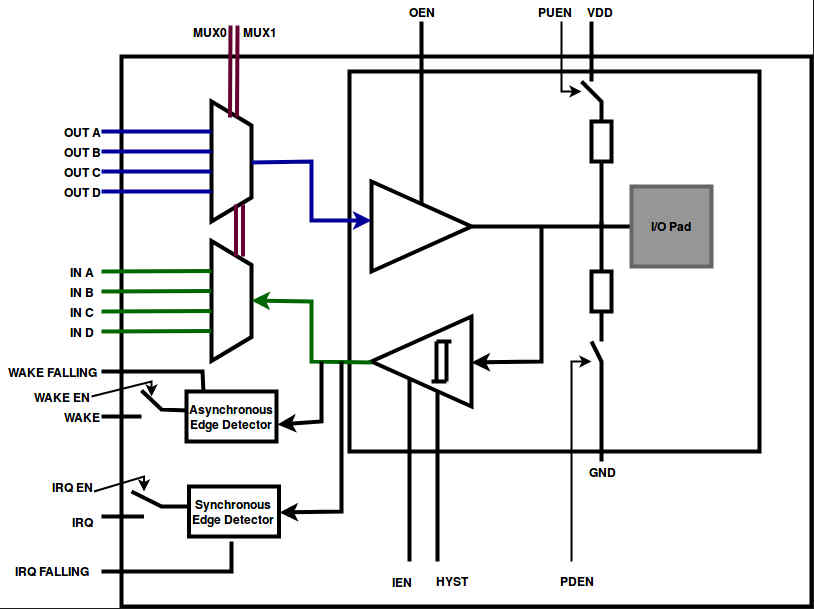
\includegraphics[height=2.5in]{../shakti/m_class/mygpiomux.jpg}\\
  {\bf 4-in, 4-out, pullup/down, hysteresis, edge-detection}
 \end{center}
}


\frame{\frametitle{Summary}

 \begin{itemize}
   \item TODO
  \end{itemize}
}


\frame{
  \begin{center}
    {\Huge The end\vspace{20pt}\\
		   Thank you\vspace{20pt}\\
		   Questions?\vspace{20pt}
	}
  \end{center}
  
  \begin{itemize}
	\item http://libre-riscv.org/shakti/m\_class/pinmux/
  \end{itemize}
}


\end{document}
